%% BrainHybridNet -- manuscript for Neural Computing and Applications (Springer Nature)
%% Template: Springer Nature LaTeX template (sn-jnl.cls), numbered references (sn-mathphys-num).
%% Compile on Overleaf: New Project -> Templates -> "Springer Nature LaTeX Template", then
%% replace its sample .tex with this file and add references.bib and figures/. See README.md.
%%
%% STATUS: NOT SUBMITTABLE YET. Every \tbd{} marks a number that must come from experiments
%% (src/evaluate.py, src/stats.py). Do not fill them with estimates.

\documentclass[pdflatex,sn-mathphys-num]{sn-jnl}

\usepackage{graphicx}
\usepackage{multirow}
\usepackage{amsmath,amssymb,amsfonts}
\usepackage{booktabs}
\usepackage{xcolor}
\usepackage{url}

\newcommand{\tbd}[1][]{\textcolor{red}{\textbf{[TBD#1]}}}


\begin{document}

\title[BrainHybridNet]{BrainHybridNet: A Lightweight Hybrid CNN--Transformer with Self-Supervised Pre-training and Uncertainty Estimation for Joint Brain Tumor Segmentation, Detection and Grading from Multi-Modal MRI}

\author*[1]{\fnm{Debobrato} \sur{Biswas}}\email{\tbd[: institutional e-mail]}
\author[1]{\fnm{\tbd[: co-author]} \sur{}}
\author[2]{\fnm{\tbd[: co-author]} \sur{}}

\affil*[1]{\orgdiv{Department of Computer Science and Engineering}, \orgname{Daffodil International University}, \orgaddress{\city{Dhaka}, \country{Bangladesh}}}
\affil[2]{\orgdiv{\tbd}, \orgname{\tbd}, \orgaddress{\city{\tbd}, \country{\tbd}}}

\abstract{\textbf{Purpose:} Automated analysis of brain tumors in multi-modal magnetic resonance imaging (MRI) usually relies on separate models for segmentation, detection and grading, many of which are large and report no measure of confidence.
\textbf{Methods:} We propose BrainHybridNet, a lightweight hybrid convolutional neural network (CNN)--vision transformer that segments the whole tumor, tumor core and enhancing tumor in 3D, detects tumor presence and predicts low- versus high-grade glioma in a single forward pass. A sequence-attention block and a two-stage CNN stem provide high-resolution features and skip connections; a four-layer transformer models long-range context. The encoder is pre-trained with 3D masked image modeling, Monte Carlo dropout provides voxel-wise epistemic uncertainty, and transformer attention provides spatial explanations. All baselines (3D U-Net, SegResNet, UNETR, SwinUNETR and nnU-Net) are re-trained on identical subject-level splits of BraTS 2021 (1,251 subjects).
\textbf{Results:} On the held-out test set BrainHybridNet reaches Dice scores of \tbd{} (whole tumor), \tbd{} (tumor core) and \tbd{} (enhancing tumor) with \tbd{} million parameters and \tbd{} ms per $128^3$ crop. \tbd[: grading, calibration and external-validation results].
\textbf{Conclusion:} \tbd[: one sentence on the measured accuracy--efficiency--calibration trade-off].}

\keywords{Brain tumor segmentation, Multi-modal MRI, Hybrid CNN--transformer, Masked image modeling, Uncertainty estimation, Glioma grading}

\maketitle

\section{Introduction}\label{sec:intro}

Brain tumors are among the most aggressive forms of cancer: glioblastoma (WHO grade 4) has a median overall survival of 14.6 months under standard-of-care treatment~\cite{stupp2005}. About 308,000 new cases of brain and central nervous system tumors were estimated worldwide in 2020~\cite{sung2021globocan}. Accurate delineation of the tumor sub-regions---whole tumor (WT), tumor core (TC) and enhancing tumor (ET)---is a prerequisite for surgical planning, radiotherapy targeting and response monitoring~\cite{menze2015}.

Multi-modal MRI is the standard for non-invasive brain tumor characterization. T1-weighted images show anatomy, contrast-enhanced T1 (T1ce) shows the enhancing tumor, T2-weighted images show peritumoral edema and FLAIR is sensitive to infiltrative tumor~\cite{gordillo2013}. Manual delineation takes a long time per case and varies between raters (Dice agreement of 74--85\%)~\cite{menze2015}, which motivates automated methods.

CNNs, particularly U-Net and its 3D variants, have dominated medical image segmentation since 2015~\cite{ronneberger2015,cicek2016}. Their local receptive fields limit the modeling of long-range spatial dependencies, which matter for large, irregular tumors~\cite{dosovitskiy2021}. Transformers~\cite{vaswani2017} attend to all positions at once, but pure vision transformers need large training sets and are expensive for 3D volumes~\cite{dosovitskiy2021}.

Existing methods leave several gaps:
\begin{enumerate}
\item \textbf{Single-task designs:} segmentation and grading are usually solved by separate models~\cite{havaei2017}.
\item \textbf{Data requirements:} transformer models need many labeled scans~\cite{chen2021transunet}.
\item \textbf{Missing uncertainty:} most segmentation methods report point predictions only~\cite{gal2016}.
\item \textbf{Limited interpretability:} clinical use requires explanations of model decisions~\cite{litjens2017}.
\item \textbf{Computational cost:} models with tens of millions of parameters are hard to deploy on standard workstations~\cite{ker2018}.
\end{enumerate}

We propose BrainHybridNet, which combines a CNN stem (local features) and a transformer bottleneck (global context) with self-supervised pre-training, uncertainty estimation and multi-task heads.

\subsection{Contributions}
\begin{enumerate}
\item \textbf{Lightweight hybrid architecture.} A ResNet-style CNN stem extracts local features and provides high-resolution skip connections; a vision-transformer bottleneck captures volumetric long-range dependencies with \tbd{} million parameters.
\item \textbf{3D masked image modeling on multi-modal MRI.} Following MAE~\cite{he2022mae} and SimMIM~\cite{xie2022simmim}, 75\% of 3D patches are masked and reconstructed before fine-tuning. Unlike self pre-training of a plain ViT on the target data~\cite{zhou2023selfmae}, masking is applied before the CNN stem of a hybrid encoder, and its effect on accuracy and label efficiency is measured (Section~\ref{sec:ablation}).
\item \textbf{Joint multi-task learning.} One model outputs tumor presence, WT/TC/ET masks and an LGG/HGG grade.
\item \textbf{Uncertainty via Monte Carlo dropout.} $T$ stochastic passes give a voxel-wise epistemic uncertainty map; we test whether it tracks segmentation error and how it affects calibration.
\item \textbf{Attention-based explanations.} Attention weights from the last transformer block give a saliency map, evaluated quantitatively against reference masks.
\item \textbf{Reproducible comparison.} All baselines are re-trained on identical splits and preprocessing; results include confidence intervals and paired significance tests; code, splits and weights are released.
\end{enumerate}

Section~\ref{sec:related} reviews related work, Section~\ref{sec:method} describes BrainHybridNet, Section~\ref{sec:setup} the experimental setup, Section~\ref{sec:results} the results, Section~\ref{sec:ablation} the ablations, Section~\ref{sec:discussion} the discussion and Section~\ref{sec:conclusion} concludes.

\section{Related work}\label{sec:related}

\subsection{CNN-based brain tumor segmentation}
U-Net~\cite{ronneberger2015} established encoder--decoder segmentation with skip connections, and 3D U-Net~\cite{cicek2016} extended it to volumes. SegResNet~\cite{myronenko2019}, winner of BraTS 2018, uses a residual encoder with variational auto-encoder regularization. MONAI~\cite{cardoso2022monai} provides optimized implementations of these models. nnU-Net~\cite{isensee2021nnunet} configures U-Net pipelines automatically and remains a strong baseline.

\subsection{Transformer-based methods}
The vision transformer~\cite{dosovitskiy2021} matches CNNs when trained at scale. TransUNet~\cite{chen2021transunet} uses a transformer bottleneck in a U-Net. The Swin transformer~\cite{liu2021swin} computes attention in shifted windows; SwinUNETR~\cite{tang2022swinunetr} applies it to 3D brain tumor segmentation, UNETR~\cite{hatamizadeh2022unetr} uses a pure transformer encoder, and TransBTS~\cite{wang2021transbts} combines a 3D CNN encoder with a transformer for BraTS. These models need substantial GPU memory.

\subsection{Hybrid CNN--transformer architectures}
MedT~\cite{valanarasu2021medt} uses gated axial attention, UCTransNet~\cite{wang2022uctransnet} replaces skip connections with channel transformers and D-Former~\cite{wu2023dformer} uses dilated attention for 3D segmentation. BrainHybridNet combines an explicit CNN stem, a small transformer with learned 3D positional embeddings and a U-Net decoder in one multi-task model.

\subsection{Self-supervised learning in medical imaging}
Contrastive methods such as SimCLR~\cite{chen2020simclr} and DINO~\cite{caron2021dino} have been adapted to medical images~\cite{sowrirajan2021mococxr}. Masked autoencoders~\cite{he2022mae} learn by reconstructing a large fraction (75\%) of masked patches. Zhou et al.~\cite{zhou2023selfmae} showed that MAE self pre-training on the target dataset improves segmentation, including BraTS. Swin UNETR pre-training~\cite{tang2022swinunetr} combines several proxy tasks on CT.

\subsection{Uncertainty estimation}
Uncertainty in deep learning has been approached with Bayesian methods~\cite{neal1996}, deep ensembles~\cite{lakshminarayanan2017} and Monte Carlo dropout~\cite{gal2016}. Nair et al.~\cite{nair2020} found that uncertain regions in multiple-sclerosis lesion segmentation coincide with errors, and Roy et al.~\cite{roy2018} used Monte Carlo sampling for segmentation quality control.

\subsection{Glioma grading}
The 2021 WHO classification combines histological and molecular markers~\cite{louis2021who}. MRI-based grading and molecular prediction have been studied with radiomics~\cite{zhou2018radiomics} and CNNs~\cite{chang2018idh}, typically as pipelines separate from segmentation.

\section{Method}\label{sec:method}

\subsection{Overview}
Figure~\ref{fig:arch} shows BrainHybridNet. It consists of (1) a sequence-attention block and CNN stem, (2) a transformer encoder on the CNN features, (3) a U-Net decoder fusing the CNN skip features and (4) task heads for segmentation, detection and grading. An optional masked-image-modeling stage pre-trains the encoder.

\begin{figure*}[t]
\centering
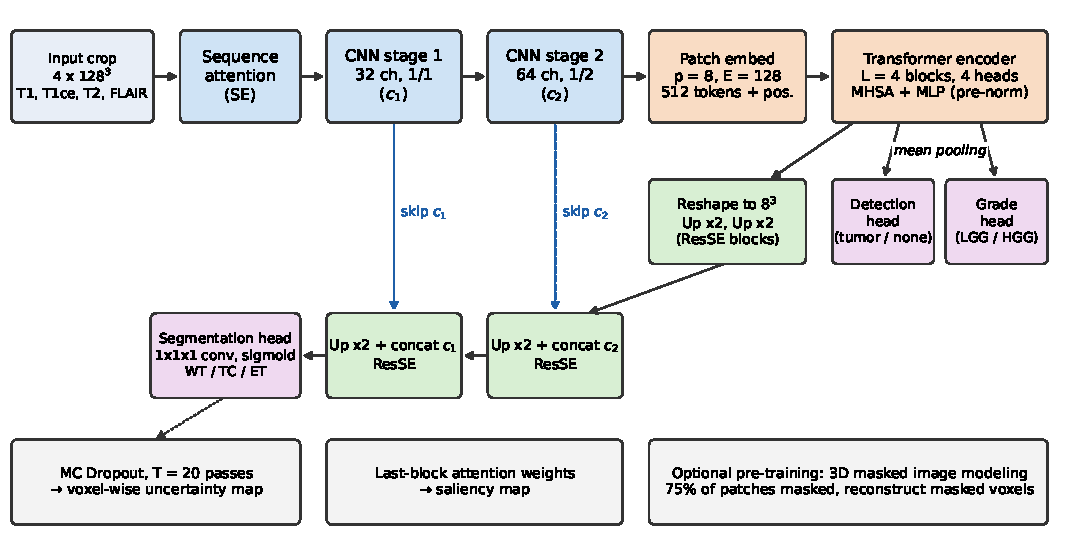
\includegraphics[width=0.95\textwidth]{figures/fig1_architecture.pdf}
\caption{BrainHybridNet. A squeeze-and-excitation block weights the four MRI sequences; a two-stage CNN stem produces skip features $c_1$ and $c_2$; 512 tokens from $8^3$ patches of $c_2$ pass through four transformer blocks. Mean-pooled tokens feed the detection and grade heads; the decoder upsamples the token grid and fuses $c_2$ and $c_1$ before the WT/TC/ET segmentation head. Monte Carlo dropout gives an uncertainty map and last-block attention a saliency map.}
\label{fig:arch}
\end{figure*}

\subsection{Input preprocessing}
The input is $\mathbf{X}\in\mathbb{R}^{B\times4\times D\times H\times W}$. BraTS 2021 volumes are skull-stripped, co-registered to the SRI24 atlas and resampled to 1\,mm isotropic resolution~\cite{baid2021brats}, so no further registration is applied. Each sequence is z-score normalized over non-zero (brain) voxels and cropped to the brain bounding box. Training uses random $128^3$ crops; with probability 0.66 a crop is centered on a random tumor voxel. Inference on whole volumes uses sliding windows of the same size with 50\% overlap and Gaussian weighting.

\subsection{Sequence attention and CNN stem}
A squeeze-and-excitation block re-weights the four sequences. The CNN stem has two stages without max-pooling:
\begin{align}
c_1 &= \mathrm{ReLU}(\mathrm{BN}(\mathrm{Conv3D}_{3,1}(\mathbf{X})))\in\mathbb{R}^{B\times32\times D\times H\times W},\\
c_2 &= \mathrm{ReLU}(\mathrm{BN}(\mathrm{Conv3D}_{3,2}(c_1)))\in\mathbb{R}^{B\times64\times\frac{D}{2}\times\frac{H}{2}\times\frac{W}{2}},
\end{align}
where the subscripts give kernel size and stride. $c_1$ and $c_2$ are the decoder's skip connections.

\subsection{Transformer encoder}
A strided convolution splits $c_2$ into non-overlapping $8^3$ patches, giving $N=\frac{D}{16}\frac{H}{16}\frac{W}{16}$ tokens of dimension $E=128$ ($N=512$ for a $128^3$ crop), to which learned positional embeddings $\mathbf{P}\in\mathbb{R}^{1\times N\times E}$ are added:
\begin{equation}
z_0=\mathrm{Flatten}(\mathrm{Conv3D}_{8,8}(c_2))^\top+\mathbf{P}.
\end{equation}
$L=4$ pre-norm transformer blocks~\cite{vaswani2017,ba2016layernorm} with 4 heads, MLP ratio 4, GELU~\cite{hendrycks2016gelu} and dropout 0.1 follow:
\begin{equation}
z'_l=z_l+\mathrm{MHSA}(\mathrm{LN}(z_l)),\qquad z_{l+1}=z'_l+\mathrm{MLP}(\mathrm{LN}(z'_l)),
\end{equation}
and a final layer normalization gives $z_L\in\mathbb{R}^{B\times N\times E}$.

\subsection{Masked image modeling pre-training}
Pre-training follows SimMIM~\cite{xie2022simmim} in 3D. A fraction $\rho=0.75$ of token positions is masked at random. The corresponding $16^3$ input regions are zeroed before the CNN stem, so masked content cannot leak through the convolutions, and masked tokens are replaced by a learned mask embedding. A linear head maps each output token to the $4\times16^3$ voxels of its region. The loss is the mean squared error to per-patch normalized targets over the masked set $\mathcal{M}$:
\begin{equation}
\mathcal{L}_{\mathrm{MIM}}=\frac{1}{|\mathcal{M}|}\sum_{i\in\mathcal{M}}\frac{\lVert\hat{x}_i-\mathrm{norm}(x_i)\rVert^2}{4\cdot16^3}.
\end{equation}
Pre-training uses only the training folds of each cross-validation split; the reconstruction head is discarded before fine-tuning.

\subsection{Decoder}
The tokens are reshaped to $z_{\mathrm{vol}}\in\mathbb{R}^{B\times E\times\frac{D}{16}\times\frac{H}{16}\times\frac{W}{16}}$ and passed through 3D dropout (0.1). Three upsampling stages (stride-2 transposed convolution followed by a residual squeeze-and-excitation block, ResSE) restore the resolution of $c_2$, which is concatenated before the third ResSE block; a fourth stage upsamples to full resolution and fuses $c_1$:
\begin{align}
u&=\mathrm{ResSE}([\mathrm{Up}(\mathrm{Up}(\mathrm{Up}(z_{\mathrm{vol}}))),c_2])\in\mathbb{R}^{B\times64\times\frac{D}{2}\times\frac{H}{2}\times\frac{W}{2}},\\
d&=\mathrm{ResSE}([\mathrm{Up}(u),c_1])\in\mathbb{R}^{B\times32\times D\times H\times W}.
\end{align}

\subsection{Task heads}
\textbf{Segmentation:} a $1\times1\times1$ convolution gives three channels (WT, TC, ET), each with a sigmoid.
\textbf{Detection:} mean-pooled tokens $\bar{z}=\mathrm{mean}(z_L)$ feed $\mathrm{Linear}(E,128)\rightarrow\mathrm{ReLU}\rightarrow\mathrm{Dropout}(0.1)\rightarrow\mathrm{Linear}(128,2)$. BraTS has no tumor-free subjects, so detection is trained at crop level: a crop is positive if it contains at least 100 whole-tumor voxels.
\textbf{Grading:} $\mathrm{Linear}(E,64)\rightarrow\mathrm{ReLU}\rightarrow\mathrm{Dropout}(0.1)\rightarrow\mathrm{Linear}(64,2)$ predicts LGG versus HGG; subjects without a grade label are ignored by this loss.

\subsection{Uncertainty estimation}
At inference, batch normalization stays in evaluation mode and dropout stays active~\cite{gal2016}. $T=20$ stochastic sliding-window passes give
\begin{equation}
\mu=\frac{1}{T}\sum_{t=1}^{T}\sigma(\hat{Y}^{(t)}),\qquad \sigma^2=\frac{1}{T}\sum_{t=1}^{T}\bigl(\sigma(\hat{Y}^{(t)})-\mu\bigr)^2,
\end{equation}
where $\sigma^2$ is the voxel-wise epistemic uncertainty map.

\subsection{Training objective and optimization}
\begin{equation}
\mathcal{L}=\lambda_1\mathcal{L}_{\mathrm{seg}}+\lambda_2\mathcal{L}_{\mathrm{det}}+\lambda_3\mathcal{L}_{\mathrm{grade}},\qquad\lambda_1=0.6,\ \lambda_2=\lambda_3=0.2.
\end{equation}
$\mathcal{L}_{\mathrm{det}}$ and $\mathcal{L}_{\mathrm{grade}}$ are cross-entropy losses. $\mathcal{L}_{\mathrm{seg}}$ is the Tversky loss~\cite{salehi2017tversky}, averaged over the three region channels:
\begin{equation}
\mathrm{TL}=1-\frac{\mathrm{TP}+\epsilon}{\mathrm{TP}+\alpha\,\mathrm{FP}+\beta\,\mathrm{FN}+\epsilon},\qquad\alpha=0.3,\ \beta=0.7,
\end{equation}
which penalizes false negatives more than false positives. The loss weights were fixed before training; their sensitivity is reported in Section~\ref{sec:ablation}.

Optimization uses AdamW~\cite{loshchilov2019adamw} (learning rate $10^{-4}$, weight decay $10^{-4}$, gradient clipping at norm 1.0), 10 warm-up epochs followed by cosine decay~\cite{loshchilov2017sgdr}, 300 fine-tuning epochs and 100 pre-training epochs (learning rate $1.5\times10^{-4}$), batch size 2 with mixed precision. Augmentation: random flips along each axis ($p=0.5$), per-sequence intensity scaling (0.9--1.1) and shift ($\pm0.1$), Gaussian noise ($\sigma=0.01$, $p=0.2$). The checkpoint with the highest mean validation Dice of each fold is kept.

\section{Experimental setup}\label{sec:setup}

\subsection{Data}
\textbf{BraTS 2021}~\cite{baid2021brats}: 1,251 subjects with expert segmentations and four co-registered sequences ($240\times240\times155$ voxels at 1\,mm$^3$). Labels are background (0), necrotic core (1), edema (2) and enhancing tumor (4); WT $=1\cup2\cup4$, TC $=1\cup4$, ET $=4$.

\textbf{Splits.} A fixed subject-level hold-out test set of 15\% of subjects (\tbd[: n] subjects) is used once, for the final results. The remaining subjects form 5 cross-validation folds shared by every model, baseline and ablation; the split file is released with the code.

\textbf{Grading data.} BraTS 2021 has no histological grades. Grading is trained and evaluated on UCSF-PDGM~\cite{calabrese2022ucsfpdgm} (WHO grade for preoperative diffuse gliomas) with its own subject-level split \tbd[: confirm], which also serves as an external segmentation test set without retraining.

\subsection{Metrics}
\textbf{Segmentation:} Dice and 95th-percentile Hausdorff distance (HD95, mm) per region, sensitivity and specificity. Following BraTS, Dice $=1$ and HD95 $=0$ when prediction and reference are both empty, and HD95 $=373.13$\,mm when only one is empty.
\textbf{Detection and grading:} AUC, accuracy, balanced accuracy, sensitivity, specificity.
\textbf{Calibration and uncertainty:} voxel-level expected calibration error (15 bins) and reliability diagrams~\cite{guo2017calibration}; Spearman correlation between case-level mean uncertainty and $1-\mathrm{Dice}$.
\textbf{Efficiency:} parameters, multiply--accumulate operations, median latency per $128^3$ crop and peak GPU memory on \tbd[: GPU].
\textbf{Statistics:} mean $\pm$ standard deviation over cases and 95\% bootstrap confidence intervals (10,000 resamples); paired Wilcoxon signed-rank tests against the strongest baseline with Holm correction.
Reporting follows the CLAIM checklist~\cite{mongan2020claim} (Supplementary Material).

\subsection{Baselines and implementation}
All baselines---3D U-Net~\cite{cicek2016}, SegResNet~\cite{myronenko2019}, UNETR~\cite{hatamizadeh2022unetr}, SwinUNETR~\cite{tang2022swinunetr} (MONAI implementations~\cite{cardoso2022monai}) and nnU-Net v2~\cite{isensee2021nnunet} (default pipeline)---are re-trained by us on the same folds with the same crops, preprocessing, augmentation, loss and schedule; no numbers are copied from other publications. Models are implemented in PyTorch~\cite{paszke2019pytorch} with PyTorch Lightning~\cite{falcon2019lightning}. Experiments ran on \tbd[: hardware]; pre-training took \tbd{} h and fine-tuning \tbd{} h per fold.

\section{Results}\label{sec:results}

\subsection{Segmentation}
\begin{table*}[t]
\caption{Segmentation on the BraTS 2021 hold-out test set (\tbd{} subjects), mean $\pm$ SD. Best value per column in bold.}
\label{tab:seg}
\centering
\begin{tabular}{lccccccccc}
\toprule
Method & \multicolumn{3}{c}{Dice $\uparrow$} & \multicolumn{3}{c}{HD95 (mm) $\downarrow$} & Params (M) & GMACs & Latency (ms)\\
 & WT & TC & ET & WT & TC & ET & & & \\
\midrule
3D U-Net~\cite{cicek2016} & \tbd & \tbd & \tbd & \tbd & \tbd & \tbd & \tbd & \tbd & \tbd\\
SegResNet~\cite{myronenko2019} & \tbd & \tbd & \tbd & \tbd & \tbd & \tbd & \tbd & \tbd & \tbd\\
UNETR~\cite{hatamizadeh2022unetr} & \tbd & \tbd & \tbd & \tbd & \tbd & \tbd & \tbd & \tbd & \tbd\\
SwinUNETR~\cite{tang2022swinunetr} & \tbd & \tbd & \tbd & \tbd & \tbd & \tbd & \tbd & \tbd & \tbd\\
nnU-Net v2~\cite{isensee2021nnunet} & \tbd & \tbd & \tbd & \tbd & \tbd & \tbd & \tbd & \tbd & \tbd\\
BrainHybridNet (ours) & \tbd & \tbd & \tbd & \tbd & \tbd & \tbd & \tbd & \tbd & \tbd\\
\botrule
\end{tabular}
\footnotetext{Significance versus the strongest baseline (Wilcoxon, Holm-corrected): \tbd.}
\end{table*}

Table~\ref{tab:seg} lists the test-set results and Table~\ref{tab:cv} the cross-validation results. \tbd[: describe the measured differences only].

\begin{table}[h]
\caption{Five-fold cross-validation, mean $\pm$ SD of fold means (Dice).}
\label{tab:cv}
\centering
\begin{tabular}{lccc}
\toprule
Method & WT & TC & ET\\
\midrule
Best baseline (\tbd) & \tbd & \tbd & \tbd\\
BrainHybridNet & \tbd & \tbd & \tbd\\
\botrule
\end{tabular}
\end{table}

\subsection{Detection and grading}
\begin{table}[h]
\caption{Crop-level tumor detection (BraTS test set) and LGG/HGG grading (UCSF-PDGM test split).}
\label{tab:det}
\centering
\begin{tabular}{lccccc}
\toprule
 & Det.\ AUC & Sens. & Spec. & Grade AUC & Grade bal.\ acc.\\
\midrule
BrainHybridNet & \tbd & \tbd & \tbd & \tbd & \tbd\\
\botrule
\end{tabular}
\end{table}

\subsection{Calibration and uncertainty}
\tbd[: voxel ECE with and without Monte Carlo dropout and for the baselines; reliability diagram (Fig.~2); Spearman $\rho$ between case-level uncertainty and $1-$Dice with $p$-value].

\subsection{External validation}
\tbd[: segmentation on UCSF-PDGM without retraining].

\subsection{Qualitative results}
\tbd[: Fig.~3 -- predictions, references, uncertainty and attention maps for representative successes and failures].

\section{Ablation study}\label{sec:ablation}

\begin{table}[h]
\caption{Ablations, 5-fold cross-validation on the development set (Dice).}
\label{tab:ablation}
\centering
\begin{tabular}{lcccc}
\toprule
Configuration & WT & TC & ET & Params (M)\\
\midrule
CNN only (no transformer) & \tbd & \tbd & \tbd & \tbd\\
Transformer path only (no CNN skips) & \tbd & \tbd & \tbd & \tbd\\
No sequence attention & \tbd & \tbd & \tbd & \tbd\\
Segmentation only (no multi-task) & \tbd & \tbd & \tbd & \tbd\\
No self-supervised pre-training & \tbd & \tbd & \tbd & \tbd\\
Full BrainHybridNet & \tbd & \tbd & \tbd & \tbd\\
\botrule
\end{tabular}
\footnotetext{Configuration files: abl\_cnn\_only, abl\_no\_skips, abl\_no\_se, abl\_no\_multitask, hybrid (with and without pre-training).}
\end{table}

\tbd[: masking ratio (0.25/0.5/0.75/0.9), number of transformer layers (2/4/6/8) and loss-weight sensitivity, three seeds each].

\section{Discussion}\label{sec:discussion}

\subsection{Clinical implications}
A model that segments, detects and grades in one pass could shorten reading time if its accuracy matches dedicated models; the uncertainty map is intended to direct review to ambiguous regions, which requires the correlation shown in Section~\ref{sec:results}. \tbd[: interpret the measured results].

\subsection{Pre-training and data efficiency}
\tbd[: effect of masked image modeling, including reduced-label experiments with 10\% and 25\% of labeled subjects].

\subsection{Explainability}
\tbd[: overlap or pointing-game evaluation of attention maps against reference masks].

\subsection{Limitations}
\begin{enumerate}
\item External validation is limited to \tbd{}.
\item WHO CNS5 classification uses IDH and other molecular markers~\cite{louis2021who}; the grading head uses imaging only.
\item Pre-training uses only BraTS training folds; larger unlabeled corpora may help.
\item BraTS has no tumor-free subjects, so detection is evaluated at crop level, not on healthy scans.
\item BraTS labels have known inter-rater variability~\cite{menze2015}.
\end{enumerate}

\subsection{Future work}
Federated training across hospitals, longitudinal response assessment, pediatric tumors, robustness to missing sequences, fusion with molecular data and a prospective reader study.

\section{Conclusion}\label{sec:conclusion}
We presented BrainHybridNet, a lightweight hybrid CNN--transformer for joint brain tumor segmentation, detection and grading from multi-modal MRI, with masked image modeling pre-training and Monte Carlo dropout uncertainty. \tbd[: one sentence summarizing measured accuracy, efficiency and calibration relative to the baselines]. Code, configurations, splits and weights are released to reproduce every reported number.

\backmatter

\bmhead{Supplementary information}
CLAIM checklist; per-fold results; additional qualitative examples. \tbd[: confirm contents].

\bmhead{Acknowledgements}
\tbd[: acknowledgements, or remove this heading].

\section*{Declarations}

\begin{itemize}
\item \textbf{Funding:} This research did not receive any specific grant from funding agencies in the public, commercial or not-for-profit sectors. \tbd[: confirm].
\item \textbf{Competing interests:} The authors declare no competing interests.
\item \textbf{Ethics approval and consent to participate:} Not applicable. This study uses publicly available, de-identified datasets (BraTS 2021, UCSF-PDGM) under their data-use terms; no new data were collected.
\item \textbf{Consent for publication:} Not applicable.
\item \textbf{Data availability:} BraTS 2021 is available at \url{https://www.synapse.org/#!Synapse:syn27046444}. UCSF-PDGM is available through The Cancer Imaging Archive under its data-use agreement~\cite{calabrese2022ucsfpdgm}.
\item \textbf{Materials availability:} Not applicable.
\item \textbf{Code availability:} Code, configuration files, data splits and trained weights are available at \url{https://github.com/Debobrato06/BrainTumorDetection} \tbd[: release tag / DOI, e.g. Zenodo].
\item \textbf{Author contribution:} D.B.: conceptualization, methodology, software, validation, writing -- original draft. \tbd[: co-author initials]: writing -- review and editing, visualization.
\end{itemize}

\bibliography{references}

\end{document}
